\documentclass[12pt]{article}
\usepackage[english]{babel}
\usepackage[autostyle, english = american]{csquotes}
\usepackage[letterpaper,top=2cm,bottom=2cm,left=3cm,right=3cm,marginparwidth=1.75cm]{geometry}
\usepackage{listings}
\usepackage{amsmath}
\usepackage{mathtools}
\usepackage[numbers]{natbib}
\usepackage{graphicx}
\usepackage[export]{adjustbox}
\usepackage[colorlinks=true,allcolors=blue]{hyperref}

\lstset{
basicstyle=\small\ttfamily,
columns=flexible,
breaklines=true
}
\MakeOuterQuote{"}
\numberwithin{equation}{section}

\DeclareMathOperator*{\argmax}{arg\,max}
\DeclareMathOperator*{\argmin}{arg\,min}

\title{Applying Keyboard Distance to the Noisy Channel Model for Spelling Correction}
%\author{Carson Mulvey}
\date{Carson Mulvey}

\begin{document}

\maketitle

\section{Introduction}

The aim of this exploration is to explain the mathematics involved in creating a spelling corrector. It will then detail how the adjacency matrix, a concept in graph theory, can be applied to computer keyboards in order to weight the spelling correction algorithm. Finally, it will statistically analyze the effectiveness of using the key positions of a computer keyboard to weigh a spelling correction algorithm.

\section{Main Body}

\subsection{Bayes' Rule}

To begin, let's prove an important formula in probability: Bayes' Rule. Proving Bayes' Rule will give better insight into its applications to real-life scenarios, including the spelling correction algorithm that will be introduced later. To start the proof, we will recall the formula for conditional logic, or the probability of an event $A$ given event $B$ is true:
\begin{equation} P(A|B)=\frac{P(A\cap{B})}{P(B)} \end{equation}
We can multiply the equation by $P(B)$ as such:
\begin{equation} P(A\cap{B})=P(A|B)\cdot{P(B)} \end{equation}
Also, there is nothing requiring the variables to be $A$ and $B$, respectively. Because of this, we can swap the variables, making another valid equation.
\begin{equation} P(B\cap{A})=P(B|A)\cdot{P(A)} \end{equation}
There is an additional manipulation we can make with these two equations. There is no difference between $A\cap{}B$ and $B\cap{A}$, as they both represent both $A$ and $B$ being true. The logical "and" operator here is commutative, or in other words, the variables can be swapped and the result will stay the same. Because of this, the left hand side of 2.2 and 2.3 are equal. Therefore, we can set the right hand sides equal.
\begin{equation} P(A|B)\cdot{P(B)}=P(B|A)\cdot{P(A)} \end{equation}
We are almost at Bayes' Rule! Just divide the equation by $P(B)$, leaving us with:
\begin{equation} P(A|B)=\frac{P(B|A)\cdot{P(A)}}{P(B)} \end{equation}
Bayes' Rule is very useful because it allows for expressing a conditional probability in terms of the individual probabilities, along with the "opposite" conditional. In other words, the probability of $A$ given $B$ can be found with the probability of $A$, the probability of $B$, and the probability of $B$ given $A$. There are many scenarios in which this theorem is used to find a conditional probability, one of which will be explained next.

\subsection{The Noisy Channel Model}

The basis of the logic behind a spelling corrector algorithm is the noisy channel model. The noisy channel model is a way to visualize the process of a word being spelt. When spelling a word, the noisy channel is taken between the intended word and what is spelt, which may or may not cause a spelling error.

\begin{figure}[h]
    \centering
    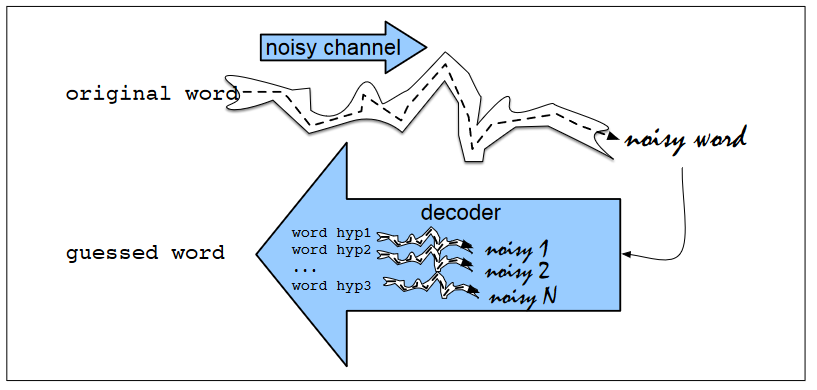
\includegraphics[width=0.8\columnwidth]{ncm.png}
    \caption{Visual of the noisy channel model}
\end{figure}

The figure above shows the application of the noisy channel model to spelling and spelling correction. The noisy channel shows the spelling of a word and how it may be incorrect after passing through the channel. Then, the decoder, which is the spelling corrector, uses a model of the noisy channel to make a prediction of the original word \cite{daniel_martin_2021}.
\\\\
The way that a noisy channel model is explained logically is through conditional probability and the argmax function. The argmax function is a function that takes every possible value for a variable, inputting it into the given expression, and outputs the value of the variable that maximizes the expression. To clarify, here is an example. Let $k$ be a variable that can be equal to $0$, $1$, or $-2$. Then, the following is true:
\begin{equation} \argmax_k{k^2}=-2 \end{equation}
This is because upon inputting $-2$ into $k^2$, we get $4$, which is larger than any other output.
With this notation in mind, we can express the noisy channel model in terms of the argmax function. Let $f$ represent the attempt to spell a word, and let $e$ be the actual word. The goal of the noisy channel model is to guess the word, $e$, given the spelling, $f$. We will call the noisy channel model's guess for the word $\hat{e}$. Then, this guess is equal to the word that is most likely based on the spelling. In other words, it is the value of $e$ with the highest probability of being the real word, given a certain $f$. This can be represented as such:
\begin{equation} \hat{e}=\argmax_e{P(e|f)} \end{equation}
Then, directly applying Bayes' Rule to the conditional probability, we get:
\begin{equation} \hat{e}=\argmax_e{\frac{P(f|e)\cdot{P(e)}}{P(f)}} \end{equation}
Finally, we know that $e$ has many possibilities, but $f$ is just the spelling for the word that we already know. This means that $f$ is constant, and therefore, $P(f)$ is constant. We can safely ignore $P(f)$ in the argmax expression because it is a positive constant.
\begin{equation} \hat{e}=\argmax_e{P(f|e)\cdot{P(e)}} \end{equation}
This is the final equation to represent the noisy channel model. While this may seem more complex than the original argmax function, the probabilities $P(f|e)$ and $P(e)$ are much easier to find than $P(e|f)$. The probability of a spelling $f$ given a word $e$ can be thought of as a likelihood that the word is misspelt in a certain way in order to get $f$. This probability will be modelled using the edit distance algorithm. The probability of $e$ on its own can be thought of a likelihood of the word $e$ being used in a sentence. The model that gives this likelihood is called the language model, which is based on the linguistic likelihood of a word being used. This exploration will use a basic language model and will not focus on its implementation. Rather, we will explain the edit distance algorithm needed for $P(f|e)$, followed by an innovative use of graph theory in an attempt to improve the algorithm's accuracy.

\subsection{Graphs, Keyboards, and the Distance Matrix}
\begin{figure}[h]
    \centering
    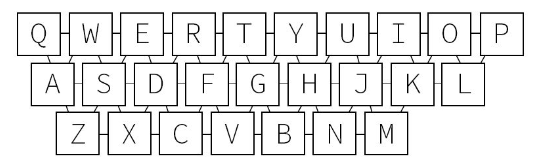
\includegraphics[width=0.8\columnwidth]{kg.png}
    \caption{A graph connecting adjacent keys on a QWERTY layout}
\end{figure}
The distance matrix of a graph is a matrix whose entries show the path length between two given nodes on a graph. By adding the distance between two keys on the graph of the QWERTY keyboard layout to a substitution, the edit distance can be weighted by the distance between keys on a keyboard. This accounts for the misspellings of words that are caused by pressing an adjacent keyboard key.
\setcounter{MaxMatrixCols}{26}
\[ 
\begin{bmatrix}
0 & 5 & 3 & 2 & 2 & 3 & 4 & 5 & 7 & 6 & 7 & 8 & 7 & 6 & 8 & 9 & 1 & 3 & 1 & 4 & 6 & 4 & 1 & 2 & 5 & 1
\end{bmatrix}
\]
\\
Take the first row of the distance matrix, for instance. The first value of the matrix is the distance from A to itself, which is 0. Then, the shortest distance from A to B on the keyboard graph is 5, and so on. A full distance matrix can be seen in the appendix, though it is very large and contains 26 by 26 values.
\subsection{The Edit Distance Algorithm}
As a reminder, the noisy channel model attempts to model a misspelling by giving probability of a word being misspelt in a specific way. The edit distance algorithm is the most common way of finding $P(f|e)$ in the channel model. The edit distance algorithm quantifies the difference between a word spelling and a potential word by counting the number of "edits" that need to be made to go from one to the other. These edits are counted as the deletion of a character, insertion of a character, or substitution of one character for another.
\\\\
As an example, let $f$ be represented by "acress." Then, if $e$ is "across," the edit distance is $1$, since the "o" being replaced by an "e" counts as a single edit. If $e$ is "cress," the edit distance is also $1$, with the single edit being the deletion of "a." However, a word like "acorn" has a much higher edit distance of $4$ through three substitutions and one insertion, which shows its lower similarity to "acress."
\cite{brill_moore_2000}
In order to be applied to the noisy channel model, probabilities can be obtained by normalizing the edit distance between $f$ and every possible $e$. Higher probabilities will correspond with lower distances, and vice versa.

\section{Conclusion}
This exploration has explained the noisy channel model, along with the use of a computer keyboard graph in order to improve the model. The rest of the noisy channel model has been implemented through a computer program. Then, the algorithm was run on test data from spelling errors on social media platform Twitter. Large spelling error data sets are often difficult to find, as they are often expensive, and many are not typed spelling errors that we desire \cite{hagiwara-mita-2020-github}. The test data resulted in 57\% success for the model with weighting by letter, and 54\% success without weighting by letter, testing with 300 cases. With improvements to the language model, both rates of success would be higher. Though insignificant now, the innovative use of graph theory to take account for keyboard distance seems to improve the accuracy of the spelling correction.

\newpage
\bibliographystyle{plainnat}
\bibliography{math_ia}

\newpage
\section{Appendix}
\appendix
\chapter{Keyboard Distance Matrix}
\setcounter{MaxMatrixCols}{26}
\[ 
\begin{bmatrix}
0 & 5 & 3 & 2 & 2 & 3 & 4 & 5 & 7 & 6 & 7 & 8 & 7 & 6 & 8 & 9 & 1 & 3 & 1 & 4 & 6 & 4 & 1 & 2 & 5 & 1 \\
5 & 0 & 2 & 3 & 4 & 2 & 1 & 1 & 3 & 2 & 3 & 4 & 2 & 1 & 4 & 5 & 6 & 3 & 4 & 2 & 2 & 1 & 5 & 3 & 2 & 4 \\
3 & 2 & 0 & 1 & 2 & 1 & 2 & 3 & 5 & 4 & 5 & 6 & 4 & 3 & 6 & 7 & 4 & 2 & 2 & 2 & 4 & 1 & 3 & 1 & 3 & 2 \\
2 & 3 & 1 & 0 & 1 & 1 & 2 & 3 & 5 & 4 & 5 & 6 & 5 & 4 & 6 & 7 & 3 & 1 & 1 & 2 & 4 & 2 & 2 & 1 & 3 & 2 \\
2 & 4 & 2 & 1 & 0 & 2 & 3 & 4 & 5 & 5 & 6 & 7 & 6 & 5 & 6 & 7 & 2 & 1 & 1 & 2 & 4 & 3 & 1 & 2 & 3 & 2 \\
3 & 2 & 1 & 1 & 2 & 0 & 1 & 2 & 4 & 3 & 4 & 5 & 4 & 3 & 5 & 6 & 4 & 1 & 2 & 1 & 3 & 1 & 3 & 2 & 2 & 3 \\
4 & 1 & 2 & 2 & 3 & 1 & 0 & 1 & 3 & 2 & 3 & 4 & 3 & 2 & 4 & 5 & 5 & 2 & 3 & 1 & 2 & 1 & 4 & 3 & 1 & 4 \\
5 & 1 & 3 & 3 & 4 & 2 & 1 & 0 & 2 & 1 & 2 & 3 & 2 & 1 & 3 & 4 & 6 & 3 & 4 & 2 & 1 & 2 & 5 & 4 & 1 & 5 \\
7 & 3 & 5 & 5 & 5 & 4 & 3 & 2 & 0 & 1 & 1 & 2 & 2 & 2 & 1 & 2 & 7 & 4 & 6 & 3 & 1 & 4 & 6 & 6 & 2 & 7 \\
6 & 2 & 4 & 4 & 5 & 3 & 2 & 1 & 1 & 0 & 1 & 2 & 1 & 1 & 2 & 3 & 7 & 4 & 5 & 3 & 1 & 3 & 6 & 5 & 2 & 6 \\
7 & 3 & 5 & 5 & 6 & 4 & 3 & 2 & 1 & 1 & 0 & 1 & 1 & 2 & 1 & 2 & 8 & 5 & 6 & 4 & 2 & 4 & 7 & 6 & 3 & 7 \\
8 & 4 & 6 & 6 & 7 & 5 & 4 & 3 & 2 & 2 & 1 & 0 & 2 & 3 & 1 & 1 & 9 & 6 & 7 & 5 & 3 & 5 & 8 & 7 & 4 & 8 \\
7 & 2 & 4 & 5 & 6 & 4 & 3 & 2 & 2 & 1 & 1 & 2 & 0 & 1 & 2 & 3 & 8 & 5 & 6 & 4 & 2 & 3 & 7 & 5 & 3 & 6 \\
6 & 1 & 3 & 4 & 5 & 3 & 2 & 1 & 2 & 1 & 2 & 3 & 1 & 0 & 3 & 4 & 7 & 4 & 5 & 3 & 2 & 2 & 6 & 4 & 2 & 5 \\
8 & 4 & 6 & 6 & 6 & 5 & 4 & 3 & 1 & 2 & 1 & 1 & 2 & 3 & 0 & 1 & 8 & 5 & 7 & 4 & 2 & 5 & 7 & 7 & 3 & 8 \\
9 & 5 & 7 & 7 & 7 & 6 & 5 & 4 & 2 & 3 & 2 & 1 & 3 & 4 & 1 & 0 & 9 & 6 & 8 & 5 & 3 & 6 & 8 & 8 & 4 & 9 \\
1 & 6 & 4 & 3 & 2 & 4 & 5 & 6 & 7 & 7 & 8 & 9 & 8 & 7 & 8 & 9 & 0 & 3 & 2 & 4 & 6 & 5 & 1 & 3 & 5 & 2 \\
3 & 3 & 2 & 1 & 1 & 1 & 2 & 3 & 4 & 4 & 5 & 6 & 5 & 4 & 5 & 6 & 3 & 0 & 2 & 1 & 3 & 2 & 2 & 2 & 2 & 3 \\
1 & 4 & 2 & 1 & 1 & 2 & 3 & 4 & 6 & 5 & 6 & 7 & 6 & 5 & 7 & 8 & 2 & 2 & 0 & 3 & 5 & 3 & 1 & 1 & 4 & 1 \\
4 & 2 & 2 & 2 & 2 & 1 & 1 & 2 & 3 & 3 & 4 & 5 & 4 & 3 & 4 & 5 & 4 & 1 & 3 & 0 & 2 & 2 & 3 & 3 & 1 & 4 \\
6 & 2 & 4 & 4 & 4 & 3 & 2 & 1 & 1 & 1 & 2 & 3 & 2 & 2 & 2 & 3 & 6 & 3 & 5 & 2 & 0 & 3 & 5 & 5 & 1 & 6 \\
4 & 1 & 1 & 2 & 3 & 1 & 1 & 2 & 4 & 3 & 4 & 5 & 3 & 2 & 5 & 6 & 5 & 2 & 3 & 2 & 3 & 0 & 4 & 2 & 2 & 3 \\
1 & 5 & 3 & 2 & 1 & 3 & 4 & 5 & 6 & 6 & 7 & 8 & 7 & 6 & 7 & 8 & 1 & 2 & 1 & 3 & 5 & 4 & 0 & 2 & 4 & 2 \\
2 & 3 & 1 & 1 & 2 & 2 & 3 & 4 & 6 & 5 & 6 & 7 & 5 & 4 & 7 & 8 & 3 & 2 & 1 & 3 & 5 & 2 & 2 & 0 & 4 & 1 \\
5 & 2 & 3 & 3 & 3 & 2 & 1 & 1 & 2 & 2 & 3 & 4 & 3 & 2 & 3 & 4 & 5 & 2 & 4 & 1 & 1 & 2 & 4 & 4 & 0 & 5 \\
1 & 4 & 2 & 2 & 2 & 3 & 4 & 5 & 7 & 6 & 7 & 8 & 6 & 5 & 8 & 9 & 2 & 3 & 1 & 4 & 6 & 3 & 2 & 1 & 5 & 0
\end{bmatrix}
\]

\chapter{Spelling Corrector Program}
\begin{lstlisting}[language=Python]
import pandas as pd
import edit_distance as editd
import math, numpy

def process_dict(input, dict, weighted):
    total_words = 0
    ndict = {}
    for i in dict:
        if (abs(len(i) - len(input))) < 3 and i.isalpha():
            total_words += dict[i]
            ndict[i] = dict[i]
    for i in ndict:
        ndict[i] = math.log10(ndict[i]/total_words) - 5 * editd.edit_distance(input, i, weighted)
    return ndict

def run_test_cases(weighted):
    unigram = pd.read_csv('unigram.csv',index_col=0,squeeze=True).to_dict()
    test_cases = pd.read_csv('tc_small.csv',squeeze=True).to_numpy()

    correct = 0
    for spelling, word in test_cases:
        prob = process_dict(spelling, unigram, weighted)
        correction = list(prob.keys())[list(prob.values()).index(max(prob.values()))]
        if word == correction:
            correct += 1
        print("W" if weighted else "UW", spelling, "->", correction, word, correct)

    return correct

if __name__ == "__main__":
    weighted_correct = run_test_cases(True)
    unweighted_correct = run_test_cases(False)
    print("Weighted:", str(weighted_correct))
    print("Unweighted:", str(unweighted_correct))
\end{lstlisting}

\end{document}